\documentclass[a4paper,10pt]{beamer}
\usepackage[utf8x]{inputenc}
\usepackage[T1]{fontenc}
\usepackage[french]{babel}
\usepackage{hyperref,graphicx,multicol,eurosym,tabularx,color}
\usetheme{Berkeley}
\setbeamercolor{structure}{fg=cyan!60!black}
\setbeamertemplate{navigation symbols}{\large \insertframenumber /\inserttotalframenumber}
\newcolumntype{M}[1]{>{\centering\arraybackslash}m{#1}}

\title{Création d'objets 3D à partir de dessins 2D}
\author[Groupe 3INFO]{Aurélien Fontaine, Manutea Huang,
\\ Etienne Geantet, Arnaud Martin}
\institute[INSA de Rennes]{Institut National des Sciences Appliquées de Rennes}
\date{\today}

\begin{document}
	
	\begin{frame}
		\begin{titlepage}
			\centerline{
\includegraphics[scale=0.1]{images/logos/logoINSA.jpg}}
			\centerline{Encadrants : François Lehericey et Bertrand Coüasnon}	
		\end{titlepage}
	\end{frame}
	
	\section{Introduction}
	
	\begin{frame}{Introduction}
		\begin{itemize}
		\item Un projet proposé par les chercheurs de l'Irisa.
		\end{itemize}
		\centerline{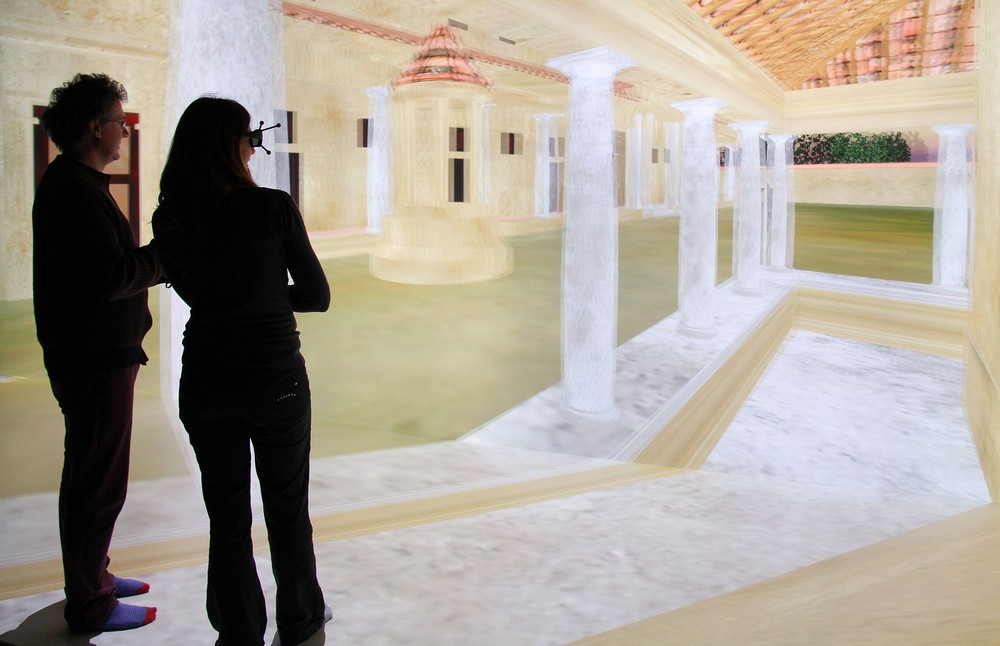
\includegraphics[scale=0.25]{images/intro/Immersia.jpg}}
		\centerline{Comment meubler rapidement une scène de réalité}
		\centerline{virtuelle avec divers objets 3D ?}
	\end{frame}
	
	\begin{frame}{Objectifs du projet}
		Contexte:
		\begin{itemize}
			\item Recherches sur la physique des objets 3D en réalité virtuelle.
			\item Besoin: Créer rapidement des modèles 3D pour les tests.
		\end{itemize}
		Problème:
			\begin{itemize}
				\item Créer un objet 3D prend beaucoup de temps (au moins 1h pour un artiste).
				\item Or dans ce cas, pas besoin d'objets complexes et esthétiques !
			\end{itemize}
		Notre projet:
		\begin{itemize}
		\item Permettre la \textbf{création rapide} d'objets simples à partir de dessins 2D.
		\item L'application met l'accent sur la \textbf{simplicité} d'utilisation et \textbf{l'ergonomie} plutôt que sur la qualité graphique des modèles.
		\end{itemize}
			\centerline{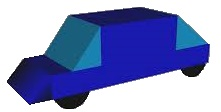
\includegraphics[scale=0.3]{images/intro/car.jpg}}
	\end{frame}
	
	\begin{frame}{Sommaire}
		\tableofcontents
	\end{frame}
	
	\section{Cahier des charges}
	
	\begin{frame}{Cahier des charges}
		Notre projet doit respecter les contraintes suivantes:
		\begin{itemize}
			\item Fonctionne sur tablette.
			\item Création d'objets 3D grâce à une suite de dessins à main levée.
			\item L'utilisateur disposera de plusieurs outils de dessin, afin de varier ses créations.
			\item L'application transforme ces dessins en objets 3D (ajout de la profondeur)
			\item L'objet final est constitué de plusieurs objets ainsi créés.
			\item L'application doit rester ergonomique, et utilisable intuitivement par tous.
			\item L'objet final peut finalement être exporté vers un serveur Unity.
		\end{itemize}
	\end{frame}
	
	\section{Etat de l'art}
	
	\begin{frame}{Quelle technologie utiliser ?}
		 Des moteurs de jeu :
		\centerline{
\includegraphics[height=75pt]{images/techno/unity-logo.png}
			
\includegraphics[height=75pt]{images/techno/UE3_logo.png}
			
\includegraphics[height=75pt]{images/techno/CryENGINE3-Logo.png}}
		\medbreak
		\begin{tabular}{l l}
			Une API : & Un logiciel de modélisation :\\
			
\includegraphics[height=75pt]{images/techno/opengl-logo.jpg} & 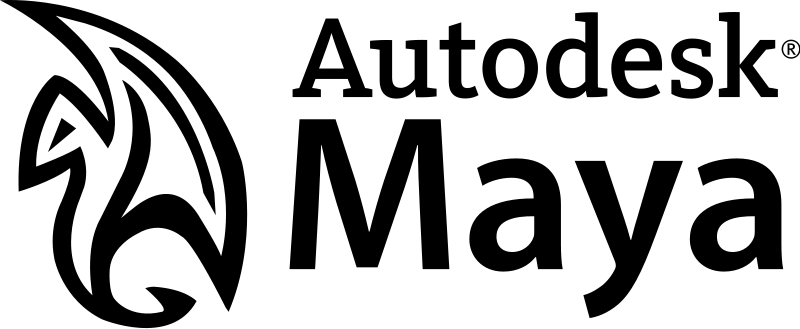
\includegraphics[height=60pt]{images/techno/auto.png}
		\end{tabular}
		
	\end{frame}
	
		\begin{frame}{Un comparatif}
			\begin{tabular}{|M{45pt}|M{40pt}|M{45pt}|M{75pt}|M{30pt}|}
				\hline
				\textbf{Software} & \textbf{Facile à apprendre} & \textbf{Manipule de nombreux objets} & \textbf{Prix} & \textbf{Aide pour tablettes}\\
				\hline
				\textit{OpenGl} & \color{red}{$\times$} & \color{orange}{$\sim$} & \color{green}{0\euro} & \color{red}{$\times$}\\
				\hline
				\textit{Autodesk Maya} & \color{red}{$\times$} & \color{green}{\checkmark} & \color{red}{\$185.00/mois} & \color{orange}{$\sim$}\\
				\hline
				\textit{Unreal Engine} & \color{green}{\checkmark} & \color{green}{\checkmark} & \color{orange}5 \% & \color{red}{$\times$}\\
				\hline
				\textit{CryEngine} & \color{green}{\checkmark} & \color{green}{\checkmark} & \color{orange}{9.99\euro/mois} & \color{orange}{$\sim$}\\
				\hline
				\textit{Unity} & \color{green}{\checkmark} & \color{green}{\checkmark} & \color{green}{0\euro : licence gratuite} & \color{green}{\checkmark} \\
				\hline
			\end{tabular}
		\end{frame}
		
		\begin{frame}{Le petit plus pour Unity}
			\centerline{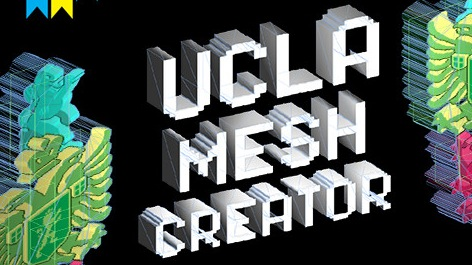
\includegraphics[height=80pt]{images/techno/ucla.jpg}}
			
			\begin{itemize}
				\item UCLA Mesh Creator : Une aide à la création d'objets en 3D à partir d'une texture
					\begin{itemize}
						\item Création uniquement en mode "Edition" de Unity
						\item Ne gère pas les trous
					\end{itemize}
				\item Gros avantage : Réutilisable facilement et sans contrainte
			\end{itemize}
			
		\end{frame}
		

	
	\section{Conception}	
		\begin{frame}{Conception}
	 		En parallèle du choix de technologie, nous avons dû réfléchir en nous basant sur deux points centraux:
		
			\begin{itemize}
				  \item Définir comment être ergonomique : découper pas à pas pour s'assurer de la simplicité à chaque instant
				  \item Diviser le logiciel en éléments les plus simples possibles et indépendants pour organiser le développement
			\end{itemize}
		\end{frame}
		
		
		\begin{frame}{Comment être ergonomique?}
				Repérage des parties pouvant poser problèmes:
				
				\begin{itemize}
					\item Comment organiser l'IHM?
					\item Comment dessiner?
					\item Comment extruder et placer la figure créée dans l'environnement 3D?
				\end{itemize}
		\end{frame}	
		
			
			\begin{frame}{Comment être ergonomique?}
				Comment organiser l'IHM?
				Problématique:
				\begin{itemize}
					\item Accueillir les futurs éléments
					\item Simplicité: peu d'options, sobre
				\end{itemize}

				\centerline{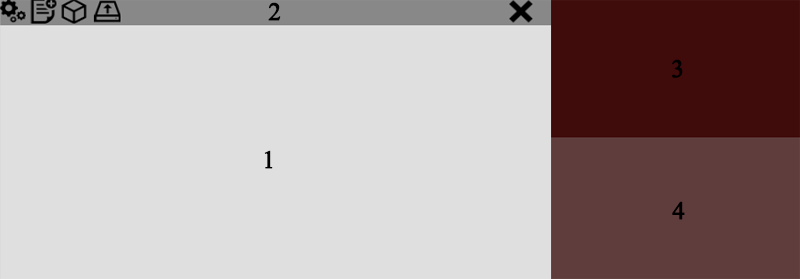
\includegraphics[scale=0.3]{images/Nono/img6.png}}
			Blender:
				\centerline{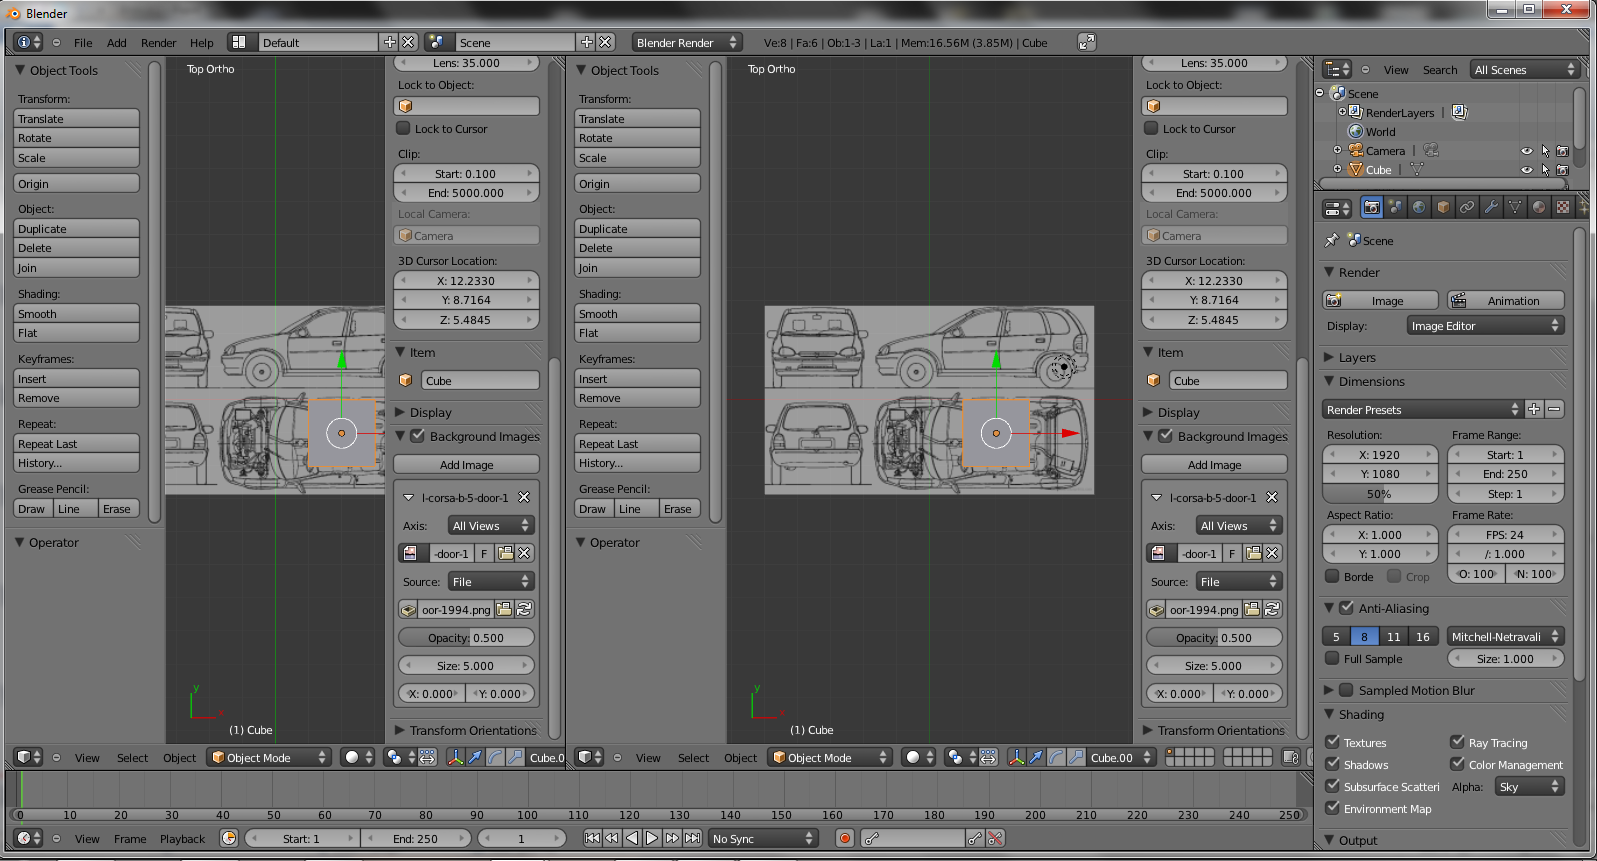
\includegraphics[scale=0.2]{images/Nono/img5.png}} 
			\end{frame}
		
		\begin{frame}{Comment être ergonomique?}

				Comment dessiner?
					\begin{itemize}
						\item Interface sobre
						\item Menu d'outils avec choix limités
					\end{itemize}
				
				\centerline{
\includegraphics[scale=0.3]{images/Nono/img1.png}} \centerline{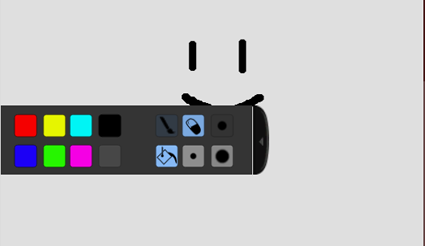
\includegraphics[scale=0.3]{images/Nono/img2.png}}
			


		\end{frame}	
		
		\begin{frame}{Comment être ergonomique?}
			
			Comment extruder et placer la figure créée dans l'environnement 3D?
			\begin{itemize}
				\item Limiter les options
				\item Découper en plusieurs étapes
				\item Transparences des autres objets
				\item Caméra globale amovible
			\end{itemize}
			
				\centerline{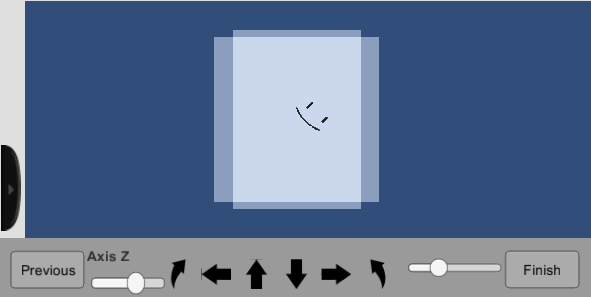
\includegraphics[scale=0.4]{images/Nono/img4.png}} 
			
			
		\end{frame}	
			
	
	\begin{frame}{Architecture logicielle} %Découpage de l'application}
		\huge Comment découper l'application?
	\end{frame}
	
	\begin{frame}{Architecture logicielle} %Découpage de l'application}
		%Archi logi Manutea
		\centerline{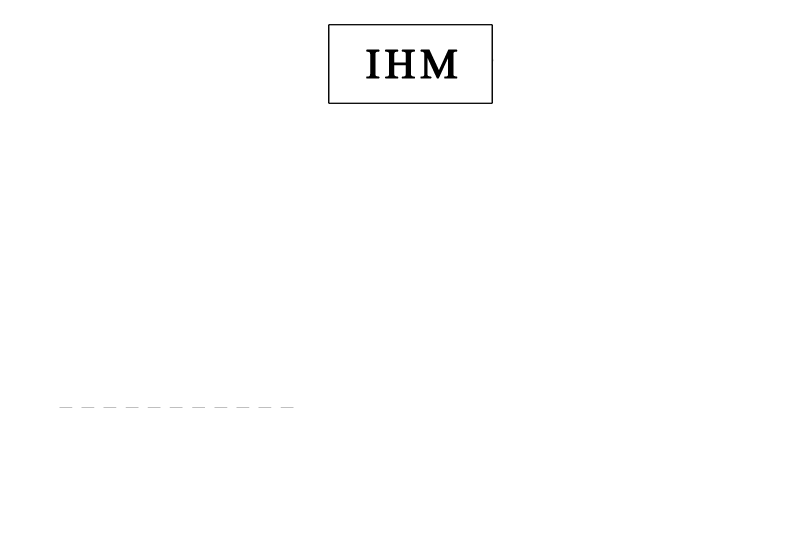
\includegraphics[scale=0.3]{images/archilogi/archi1.png}}
	\end{frame}
	\begin{frame}{Architecture logicielle} %Découpage de l'application}
		%Archi logi Manutea
		\centerline{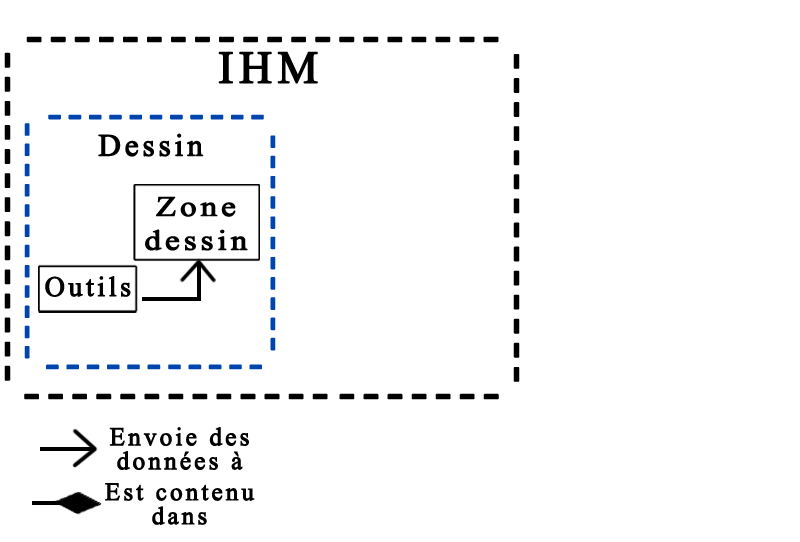
\includegraphics[scale=0.3]{images/archilogi/archi2.png}}
	\end{frame}
	\begin{frame}{Architecture logicielle} %Découpage de l'application}
		%Archi logi Manutea
		\centerline{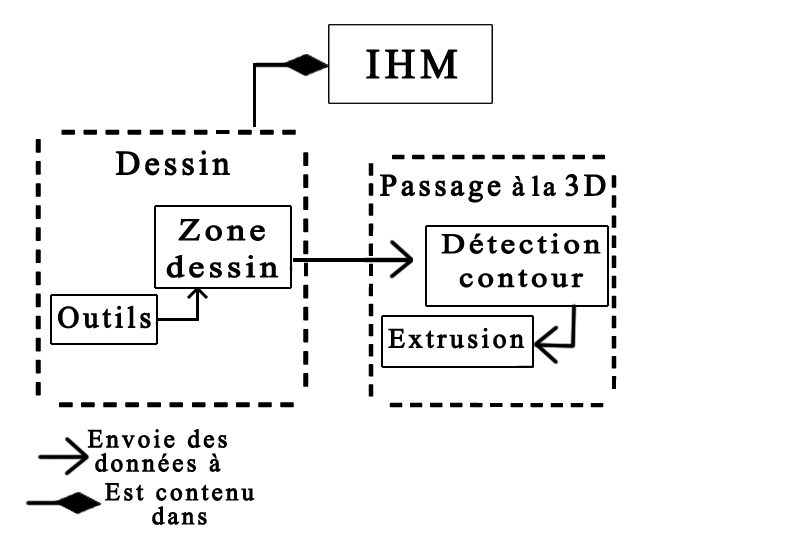
\includegraphics[scale=0.3]{images/archilogi/archi3.png}}
	\end{frame}
	\begin{frame}{Architecture logicielle} %Découpage de l'application}
		%Archi logi Manutea
		\centerline{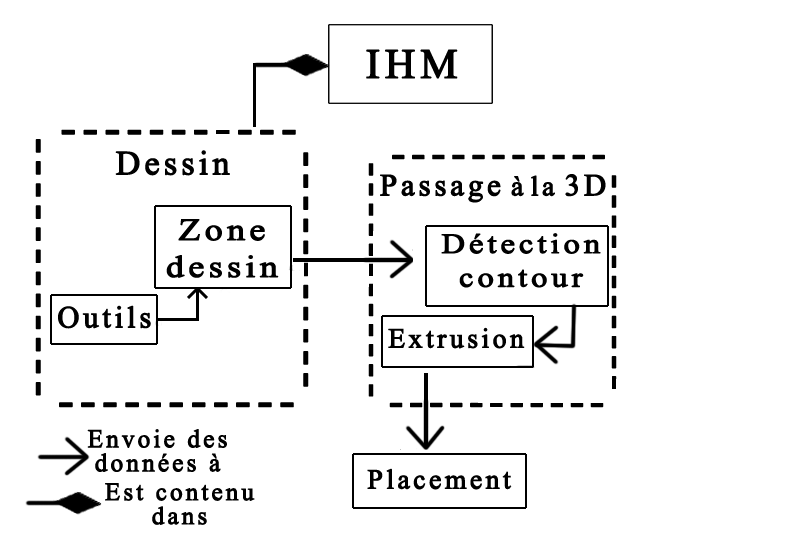
\includegraphics[scale=0.3]{images/archilogi/archi4.png}}
	\end{frame}
	\begin{frame}{Architecture logicielle} %Découpage de l'application}
		%Archi logi Manutea
		\centerline{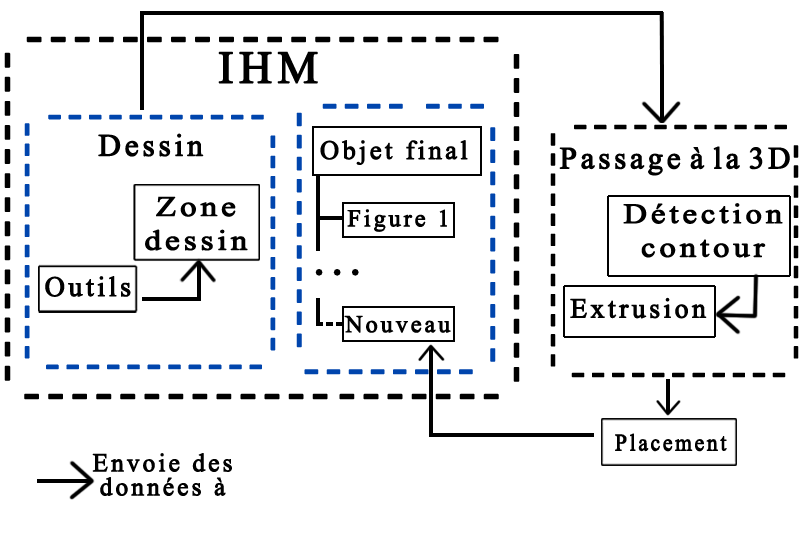
\includegraphics[scale=0.3]{images/archilogi/archi5.png}}
	\end{frame}	
			
	\section{Implémentation sous Unity}
		%Expliquer nos choix par rapports aux objectifs énoncés
			\begin{frame}{Implémentation sous Unity}
				Phase de réflexion terminée. On a déjà défini:
					\begin{itemize}
						\item Choix technologique : Unity
						\item Le fonctionnement de l'application
						\item L'architecture du logiciel
					\end{itemize}
					
				Nous avons désormais les éléments pour implémenter notre projet.
			\end{frame}
		
		
	\begin{frame}{IHM et Outils}

				\begin{itemize}
					\item Technologie Unity UI (gestion de menus)
					\item Boutons et caméras vides
					\item Facilité d'implémentation de nouveaux outils
				\end{itemize}
			
	\end{frame}
	

	
	\begin{frame}{La zone de dessin}
		Le dessin doit apparaître sur la texture de l'objet.
			\centerline{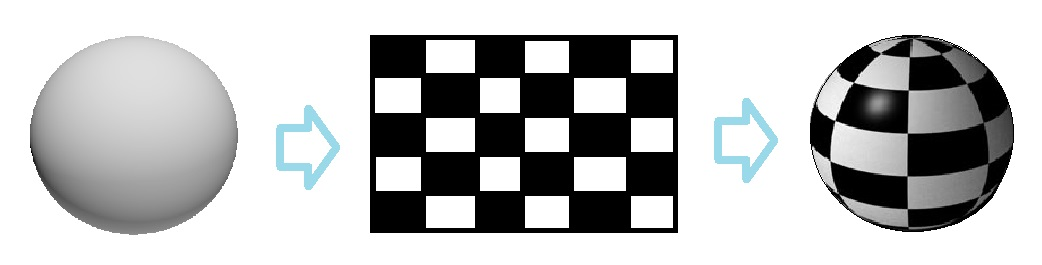
\includegraphics[scale=0.4]{images/intro/spheres.jpg}}
			
			\begin{itemize}
				\item Le plan (GameObject dans Unity) et la texture n'ont pas le même référentiel. 
				\item Pour accéder au pixel sur lequel on clique, on doit chercher le point d'intersection entre un Ray que l'on projette, et la zone de dessin.
				\item Le dessin se fait simplement en modifiant la texture aux endroits où  l'on clique.
			\end{itemize} 
		La fond de la texture doit être en alpha pour n'extruder que ce qui a été colorié.
	\end{frame}
	
	\begin{frame}{La zone de dessin}
		\begin{itemize}
		\item Unity va tester la position du doigt à chaque frame.
		Pour garder un tracé continu, on trace la droite entre le point courant et le dernier point.
		\centerline{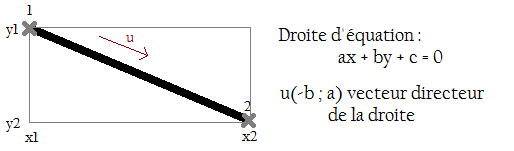
\includegraphics[scale=0.4]{images/intro/trait.png}}
		
		\item Pour le remplissage de la texture avec l'outil Bucket, on a utilisé un algorithme de remplissage par pile explicite.
	\end{itemize}
	\end{frame}
	
	\begin{frame}{L'extrusion : Définition}
		Plusieurs étapes pour passer d'une texture à un objet :
		\begin{itemize}
			\item Détection des contours du dessin
			\item Création de meshes
			\item Assemblage des meshes -> Objet 3D
			\item Application de la texture pour rendre l'objet coloré
		\end{itemize}
	
	\end{frame}
		
	\begin{frame}{L'extrusion}
		
		Le passage du dessin à l'objet 3D pour notre application :
		\begin{itemize}
			\item Extrusion faite par UCLA Mesh Creator
			\item Intégration de l'outil à notre application
		\end{itemize}
		\medbreak
		Problèmes rencontrés :
		\begin{itemize}
			\item Utilisation impossible en mode "Jeu" -> Exécutable impossible
			\item Création de nombreux fichiers inutiles pour la suite
		\end{itemize}
	\end{frame}
	
	\begin{frame}{Envoi des données}
		\centerline{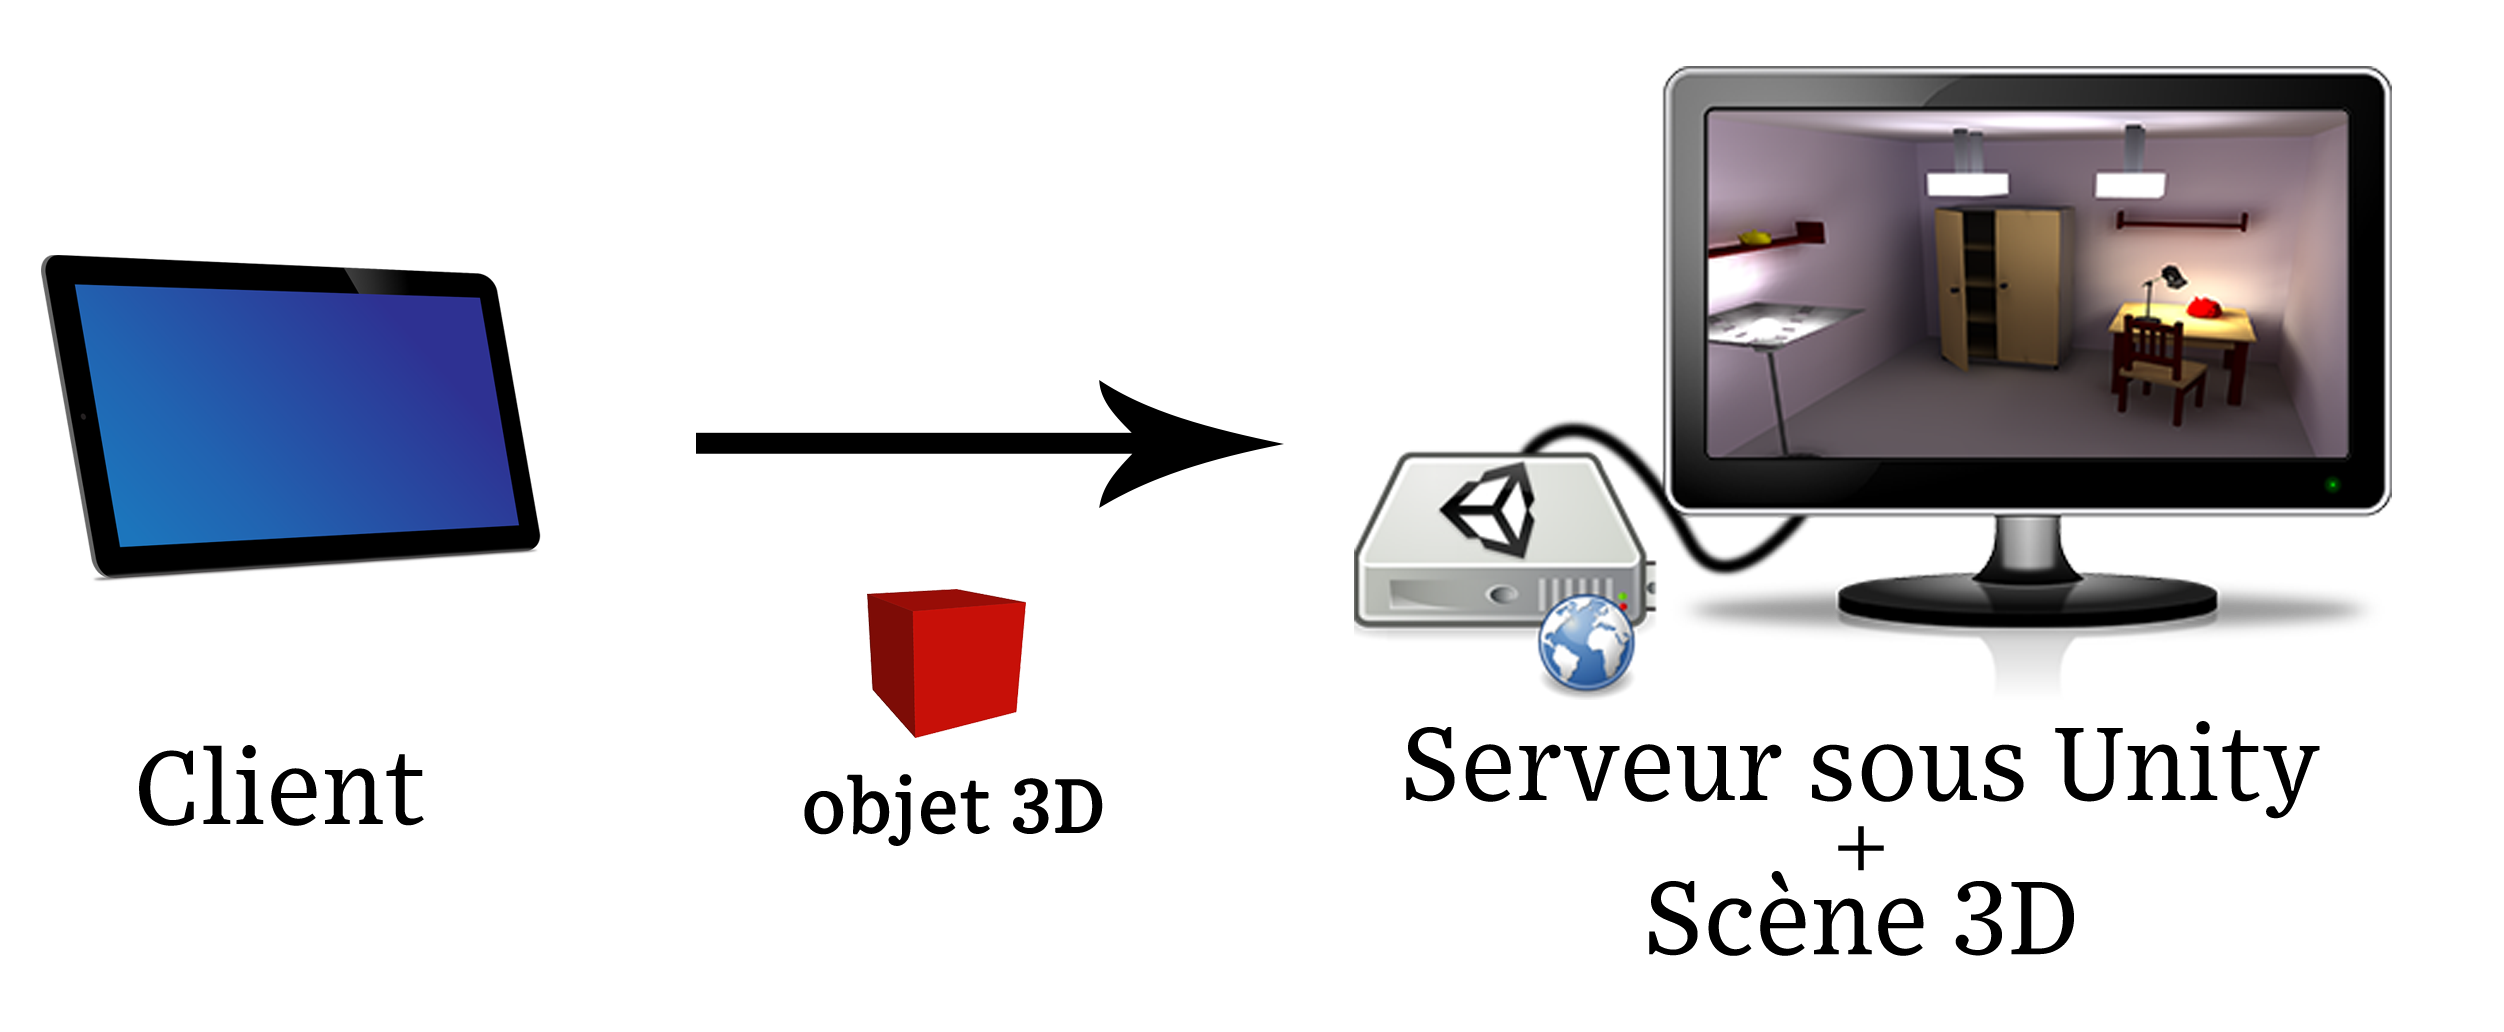
\includegraphics[height=120pt]{images/network/sending_model2.png}}
	\end{frame}
	
	
	\begin{frame}{Côté serveur}
		\centerline{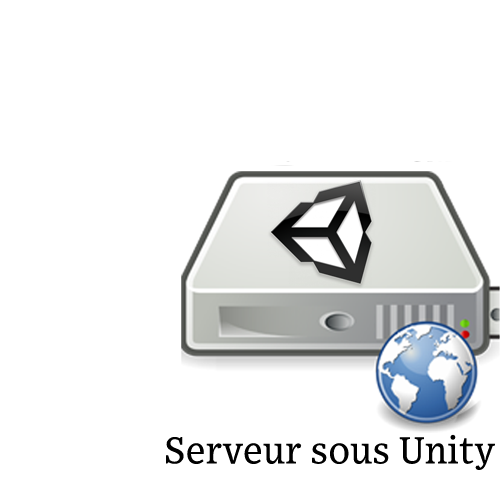
\includegraphics[height=150pt]{images/network/plugin1.png}}
		\invisible{
		\begin{itemize}	
			\item  Léger 
			\item Reçoit les données 
			\item Intégré dans la scène 3D
			\item Affiche l'objet 
		\end{itemize}	}
		
	\end{frame}
	\begin{frame}{Côté serveur}
		\centerline{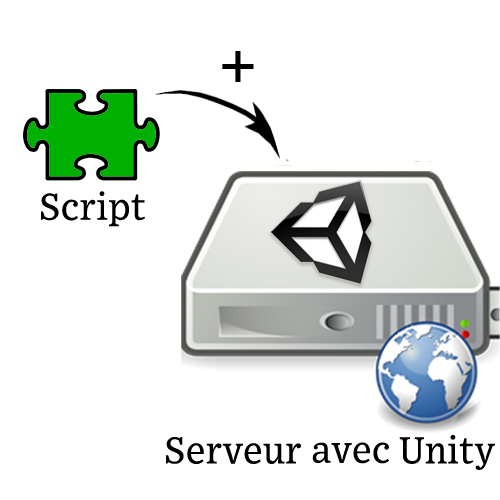
\includegraphics[height=150pt]{images/network/plugin.png}}
		\begin{itemize}	
			\item \pause Léger \pause
			\item Reçoit les données \pause
			\item Affiche l'objet 
		\end{itemize}	
		
	\end{frame}
	
	
	\begin{frame}{Socket TCP}
		\centerline{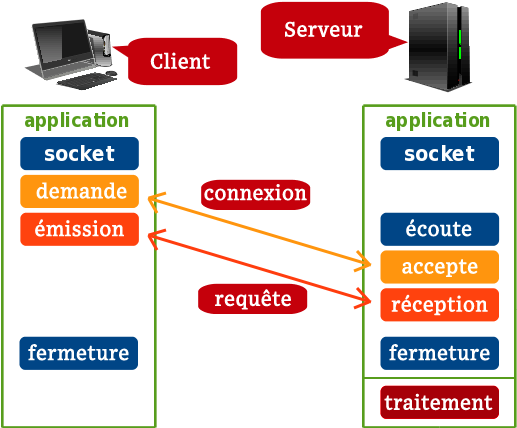
\includegraphics[height=150pt]{images/network/tcp-socket6.png}}
		\invisible{
		\begin{itemize}
			\item Dispose de classes prévues à cet effet en C\# 
			\item Documentée en C\# par Microsoft 
			\item Permet d'envoyer des octets, donc flexible
		\end{itemize}
	}
	\end{frame}
	\begin{frame}{Socket TCP}
		\centerline{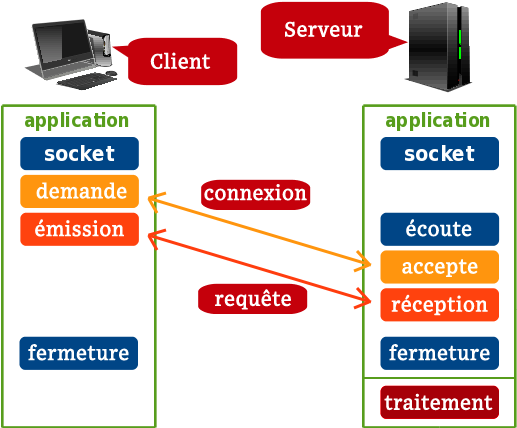
\includegraphics[height=150pt]{images/network/tcp-socket6.png}}
			\begin{itemize}
				\item Dispose de classes prévues à cet effet en C\# \pause
				\item Documentée en C\# par Microsoft \pause
				\item Permet d'envoyer des octets, donc flexible
			\end{itemize}
	\end{frame}
	
	\section{Conclusion}
	
	\begin{frame}{Notre application}
		Voici une vidéo montrant un exemple d'utilisation de notre application :
		%vidéo -> présente les points clés de notre présentation
	\end{frame}
	
	\begin{frame}{Pour résumer}
		Nous avons fait une application Unity :
		\begin{itemize}
			\item sur tablette Windows\pause
			\item Simple et rapide:\pause
		\end{itemize}
		\centerline{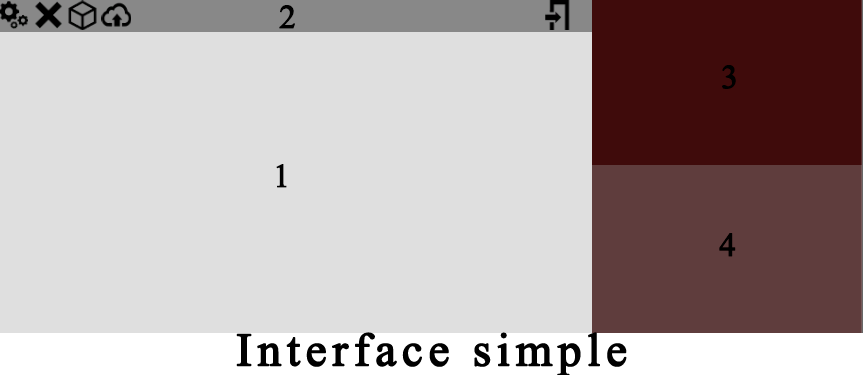
\includegraphics[height=60pt]{images/conclu/menu.png}\pause\hspace{10 mm}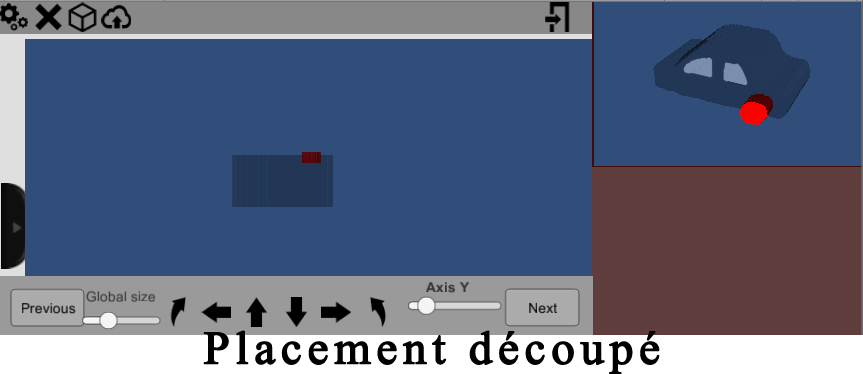
\includegraphics[height=60pt]{images/conclu/place.png}\pause}
		\begin{tabular}{lll}
			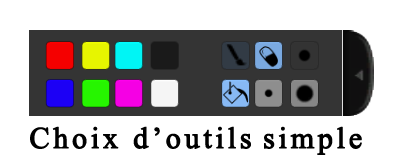
\includegraphics[height=40pt]{images/conclu/outils.png} & \pause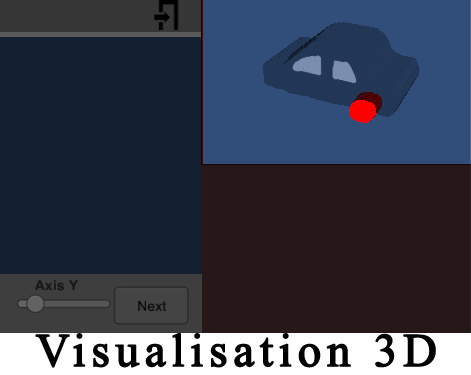
\includegraphics[height=75pt]{images/conclu/visu.png}\pause & 
\includegraphics[height=30pt]{images/conclu/export.png}
		\end{tabular}
		 
	\end{frame}
		
\end{document}
